Um ein Bild von der allgemeinen Übereinstimmung der simulierten Daten mit den tatsächlich beobachteten Daten zu erhalten wird in diesem Kapitel das Jahresmittel der simulierten und beobachteten Daten verglichen. Dadurch erhält man einen Überblick über die geographische Übereinstimmung der Regenzonen und Trockengebiete im abgebildeten Bereich.
\begin{figure}[h]
	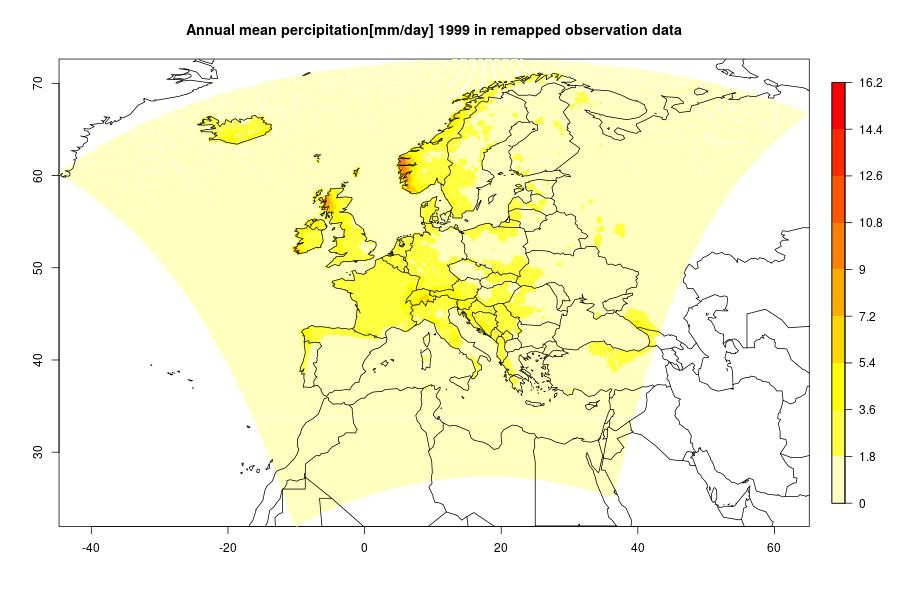
\includegraphics[width=15cm]{mean/mprs1999obs_remapped.jpg}
	\caption{Jährliches Mittel über den Niederschlag im Jahr 1999 der tatsächlich Beobachteten Daten}
	\label{fig:mobs99}
\end{figure}
\\
Zu Abb. \ref{fig:mobs99}: Man erkennt gut die starken Regenfälle an der Westküste Norwegens und Englands (bis zu 12.6 mm). Der Niederschlag an Irlands Westküste und im Alpenbereich fielen 1999 im Mittel schwach aus (bis zu 7.2mm). Über Deutschland, Frankreich und weiten Teilen Europas fielen im Schnitt 3.6-5.4 mm Regen am Tag.\\
\begin{figure}[h]
	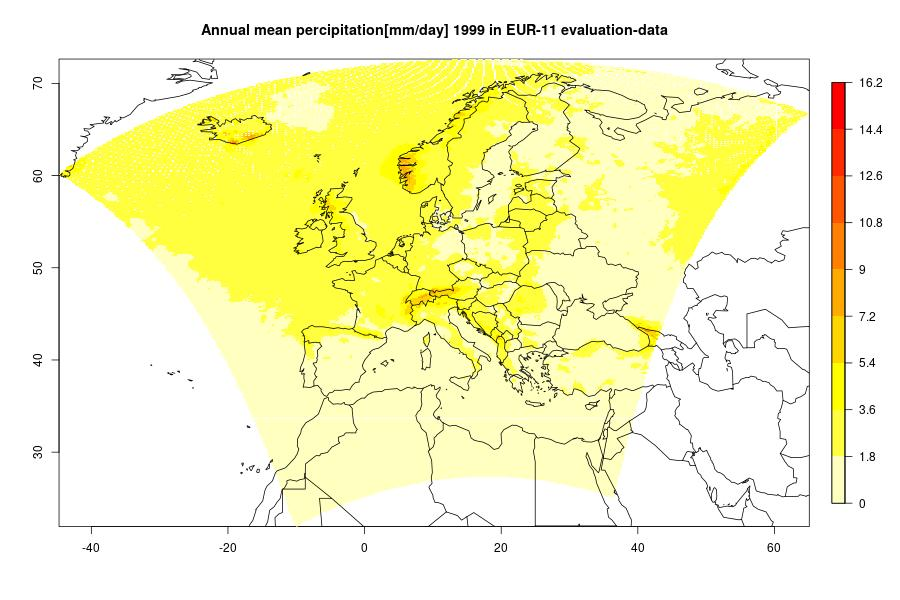
\includegraphics[width=15cm]{mean/msim1999eval.jpg}
	\caption{Jährliches Mittel über den Niederschlag im Jahr 1999 im evalualtion Datensatz von EUR-11}
	\label{fig:meval99}
\end{figure}
 \\
Zu Abb. \ref{fig:meval99}: Man sieht generell gute Übereinstimmungen an der Küste Norwegens und Englands, der Regen in Island und einigen Teilen des Alpenraumes fielen im Modell zu stark aus. Auch in Georgien am Kaukasus liefert das Modell einen zu starken Regen. Da das Klimamodell CCLM4-8-17 eine Parametrisierung der Konvektion vornimmt, ist die geringe Übereinstimmung in gebirgigen Gebieten nicht überraschend. Der Unterschied zur folgenden Abbildung \ref{fig:mhist99} ist lediglich die Quelle der Daten für das downscalen: hier wurde das CCLM mit Re-Analysedaten betrieben, im folgenden mit dem GCM MPI-ESM-LR.\\
\hfill
\begin{figure}[h]
	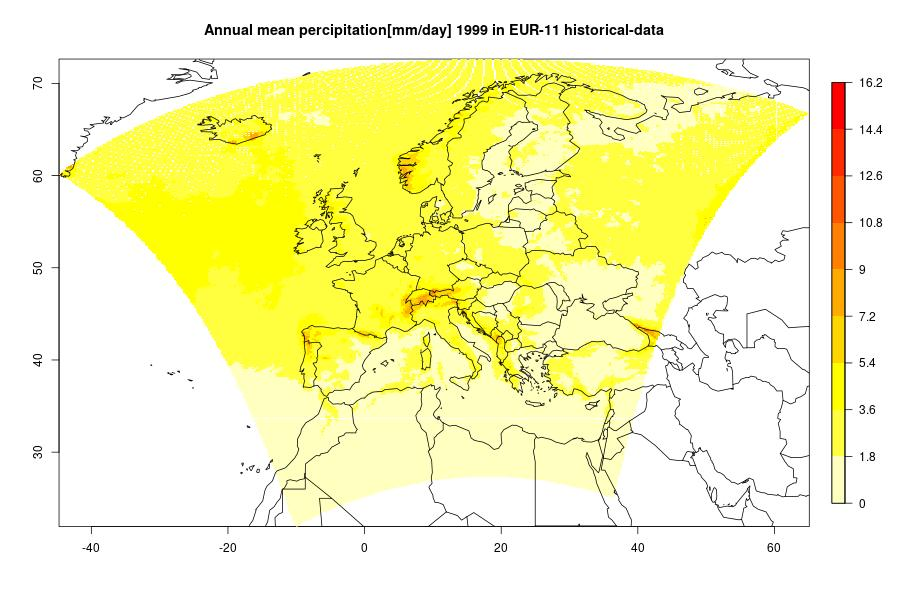
\includegraphics[width=15cm]{mean/msim1999hist.jpg}
	\caption{Jährliches Mittel über den Niederschlag im Jahr 1999 im historical Datensatz von EUR-11}
	\label{fig:mhist99}
\end{figure}
\hfill\\
Zu Abb. \ref{fig:mhist99}: Der Regen an der norwegischen Westküste fällt bei dieser Modellaufnahme um einiges schwächer aus als in der Aufnahme des Evaluation Datensatzes zuvor. Dies ist noch auffallender im Vergleich mit den Beobachtungsdaten. Mit dem Niederschlag an der britischen Westküste verhält es sich ähnlich, Auffallend sind besonders die Erscheinungen im Süden Frankreichs, wo aus unersichtlichen Gründen im Flachland um Toulouse größere Regenmengen \glqq voraus \grqq-gesagt wurden. Die Analyse des Alpenraums und des Kaukasusgebiets fallen fast gleich aus wie die im Evaluationsdatensatz (Abb. \ref{fig:meval99}). Bei dieser Herangehensweise wurde das CCLM mit dem GCM MPI-ESM-LR für die historische Periode 1999 angetrieben. Es sind darin wohl einige Abweichungen zum tatsächlichen Globalen Klima vorhanden oder aber das downscaling hat diese Erscheinungen hervorgebracht.
LLLLLLLLLLLLLLLLLLLLLLLLLLLLLLLLLLLLLLLLLLLLLLLLOOOOOOOOOOOOOOOOOOOOOOOOOOOOOOOOOKKKKKKKKKKKK Dies wird erst im Vergleich zum feineren ALP-3 ersichtlich.\hfill\\

\begin{figure}[h]
	\centering
	\begin{subfigure}[h]{0.49\textwidth}
		\centering
		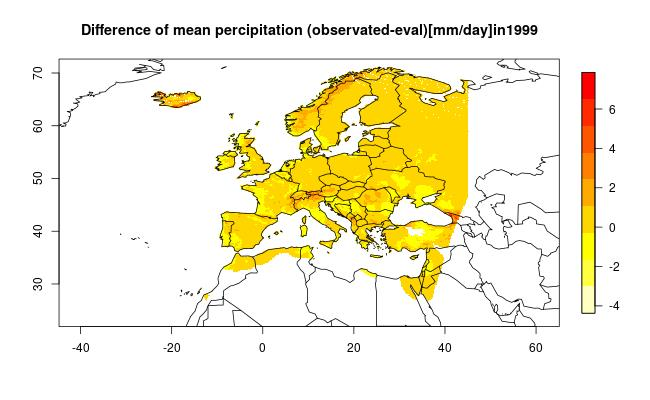
\includegraphics[width=\textwidth]{mean/1999dif_mprs_eval-obs.jpg}
		\caption{Differenz des Beobachtungsdatensatzes und des evaluation-Datensatzes}
		\label{fig:eval_dif}
	\end{subfigure}
	\begin{subfigure}[h]{0.49\textwidth}
		\centering
		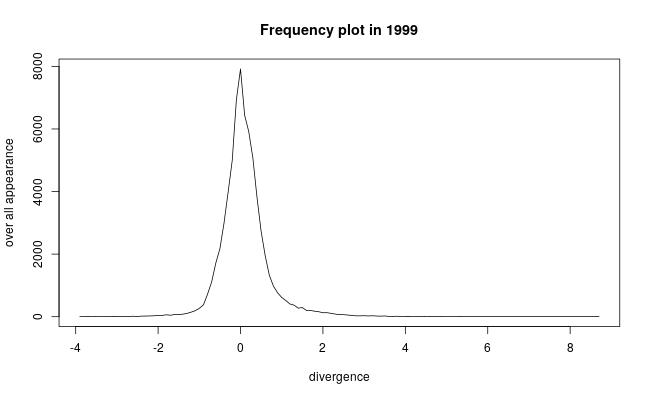
\includegraphics[width=\textwidth]{mean/1999frequenciesdif_mprs_eval-obs.jpg}
		\caption{Häufigkeit der Abweichungen über das gesamte Gitter}
		\label{fig:eval_freq_dif}
	\end{subfigure}
	\begin{subfigure}[h]{0.49\textwidth}
		\centering
		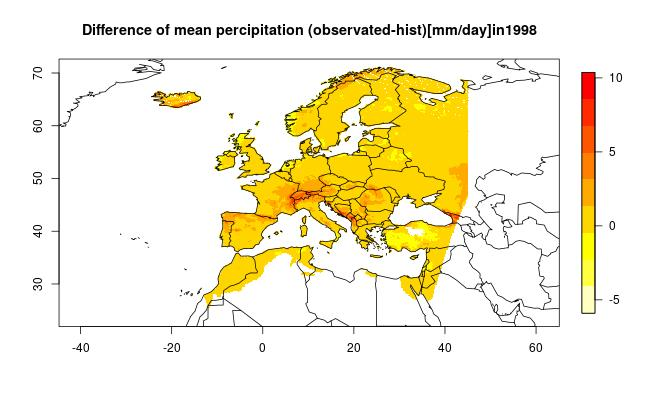
\includegraphics[width=\textwidth]{mean/1999dif_mprs_hist-obs.jpg}
		\caption{Differenz des Beobachtungsdatensatzes und des historical-Datensatzes}
		\label{fig:hist_dif}
	\end{subfigure}
	\begin{subfigure}[h]{0.49\textwidth}
		\centering
		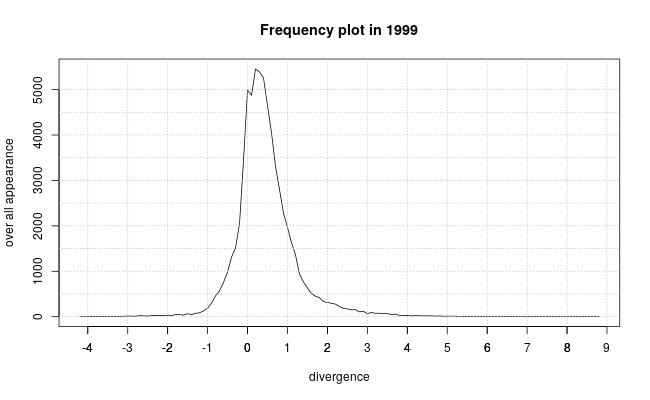
\includegraphics[width=\textwidth]{mean/1999frequenciesdif_mprs_hist-obs.jpg}
		\caption{Häufigkeit der Abweichungen über das gesamte Gitter für den historical-Datensatz}
		\label{fig:hist_freq_dif}
	\end{subfigure}
	\caption{Differenzen für den evaluation- und historical- Datensatz}
\end{figure}

\vfill
Wie man gut in Abb. \ref{fig:eval_dif} erkennen kann ist im allgemeinen über den orthographisch gediegenen Gegenden die Abweichung vom Beobachtungsdatensatz gering. Es ist gut ersichtlich, dass die Abweichungen in überwiegend gebirgigen Gegenden größer sind. Wie auch in Abb. \ref{fig:eval_freq_dif} zu sehen ist, überwiegt eine Abweichung von 0, auch wenn die Kurve leicht ins rechte verschoben ist - dies bedeutet dass mehr Niederschlage simuliert wurde als es tatsächlich gab. Der Mittelwert der Abweichungen in diesem Datensatz beträgt für das Jahr 1999 $+0.1009$.\\
Man kann auch gut erkennen, dass im historical-Datensatz (siehe Abb. \ref{fig:hist_dif}) die Abweichungen größer sind als im evaluation Datensatz, was darauf zurückzuführen ist, dass für den historical-Datensatz die Auswirkungen eines simulierten globalen Klimas auf regionale Ebene berechnet wurden, und dadurch Abweichungen zur tatsächlichen Konstellation der Atmosphäre von vornherein herrschen. Der Mittelwert der Abweichungen in diesem Datensatz beträgt für das Jahr 1999 $+0.4590$. Dies ist bedeutend höher als im evaluation-Datensatz. Man kann dies auch gut in der Abbildung \ref{fig:hist_freq_dif} erkennen, wo die maximale Häufigkeit nicht mehr über $0$ sondern über ca. $+0.3$ liegt.\\
Im folgenden sollen alle Jahre gemittelt verglichen werden um eine Allgemeinaussage über das GCM MPI-ESM-LR und das betreffende CCLM4-8-17 treffen zu können:
\begin{figure}[h]
	\begin{subfigure}[h]{0.49\textwidth}
	\centering
	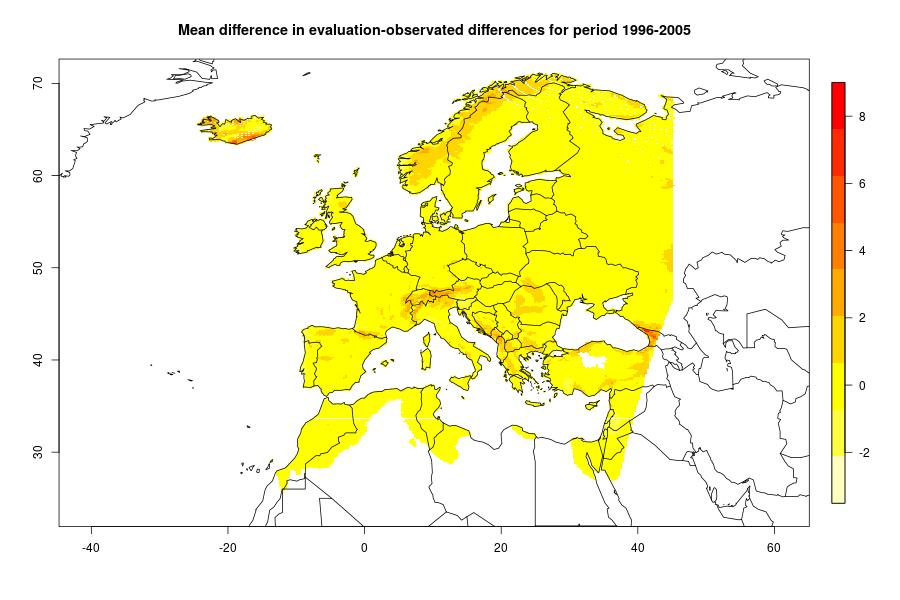
\includegraphics[width=\textwidth]{mean/dif_mean_eval.jpg}
	\caption{Gemittelte Abweichungen von den Beobachtungsdaten über die gesamte Periode für den EUR-11 Evaluations-Datensatz}
	\label{fig:mean_dif_eval}
	\end{subfigure}
	\begin{subfigure}[h]{0.49\textwidth}
		\centering
		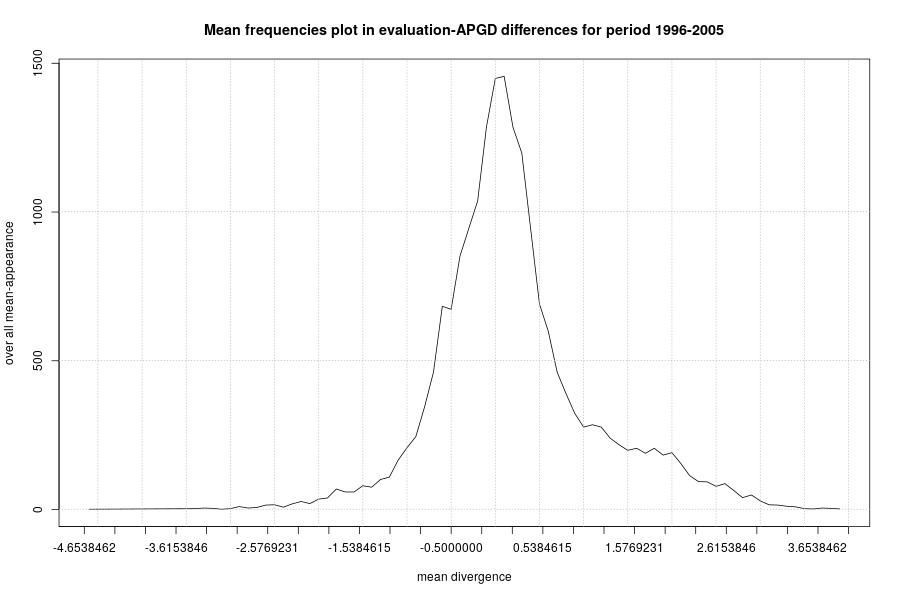
\includegraphics[width=\textwidth]{mean/frequenciesdif_mean_eval.jpg}
		\caption{Gemittelte Häufigkeit der Abweichungen von den Beobachtungsdaten über die gesamte Periode für den EUR-11 Evaluations-Datensatz}
		\label{fig:freq_mean_dif_eval}
	\end{subfigure}
	\caption{Gemittelte Abweichungen im EUR-11 evaluation-Datensatz}
\end{figure}
\begin{figure}[h]
	\begin{subfigure}[h]{0.49\textwidth}
	\centering
	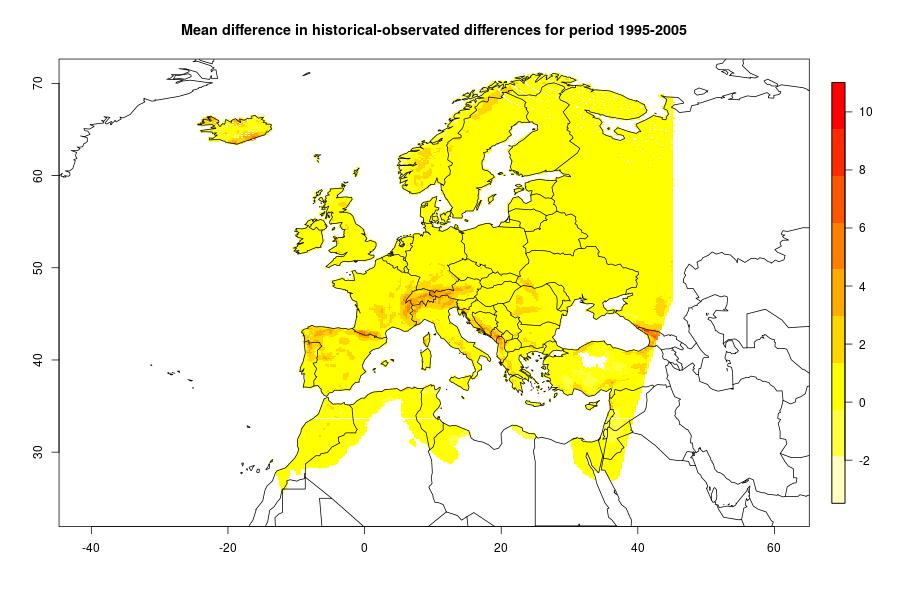
\includegraphics[width=\textwidth]{mean/dif_mean_hist.jpg}
	\caption{Gemittelte Abweichungen von den Beobachtungsdaten über die gesamte Periode für den EUR-11 historical-Datensatz}
	\label{fig:mean_dif_hist}
	\end{subfigure}
	\begin{subfigure}[h]{0.49\textwidth}
			\centering
		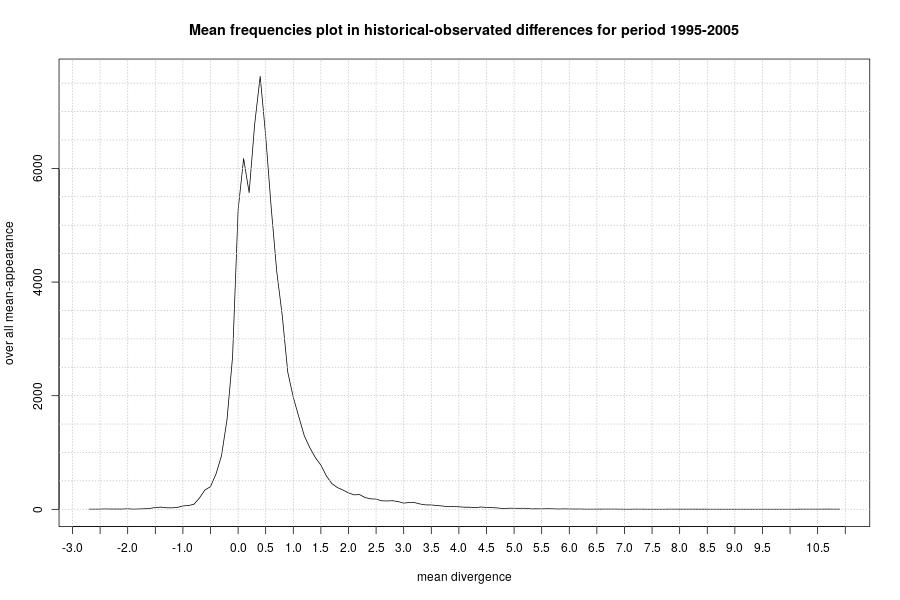
\includegraphics[width=\textwidth]{mean/frequenciesdif_mean_hist.jpg}
		\caption{Gemittelte Häufigkeit der Abweichungen von den Beobachtungsdaten über die gesamte Periode für den EUR-11  historical-Datensatz}
		\label{fig:freq_mean_dif_hist}
	\end{subfigure}
	\caption{Gemittelte Abweichungen im EUR-11 historical-Datensatz}
\end{figure}
\hfill\\
Die Abweichungen für den historical-Datensatz, die wir zuvor für das Jahr 1999 berechnet haben scheint sich im Mittel auch für die gesamte Periode abzubilden. Man erkennt beim vergleichen der Abb. \ref{fig:mean_dif_hist} und \ref{fig:hist_dif}, dass sich der Mittelwert der Verteilungskurve noch weiter ins positive verschoben hat. Man erhält eine mittlere Abweichung von $0.5568$. Es wurde also im Mittel auch zu viel Niederschlag simuliert.\\
Die gemittelten Abweichungen beim evaluation-Datensatz zeichnen sich auch dem Jahre 1999 entsprechend ab, wobei auch hier im Durchschnitt eine Verschiebung ins Positive stattgefunden hat: die höchste Häufigkeit liegt zwar immer noch über $0$ aber die mittlere Abweichung liegt bei $0.1297$ was um $0.0289	$ über dem Jahre 1999 liegt.